\documentclass[aspectratio=169]{beamer}
\usetheme{metropolis}
\usepackage{graphicx}
\usepackage{booktabs}
\usepackage{amsmath}
\usepackage{tikz}
\usepackage{xcolor}

\definecolor{accent}{HTML}{2980b9}
\definecolor{highlight}{HTML}{e74c3c}
\definecolor{success}{HTML}{27ae60}

\title{Paraphraser Fingerprinting}
\subtitle{Can We Identify the Rewriter from the Text Alone?}
\author{CS6120 Project}
\institute{Northeastern University}
\date{}

\begin{document}

% ============================================================
\begin{frame}
\titlepage
\end{frame}

% ============================================================
\begin{frame}{Motivation}

\begin{center}
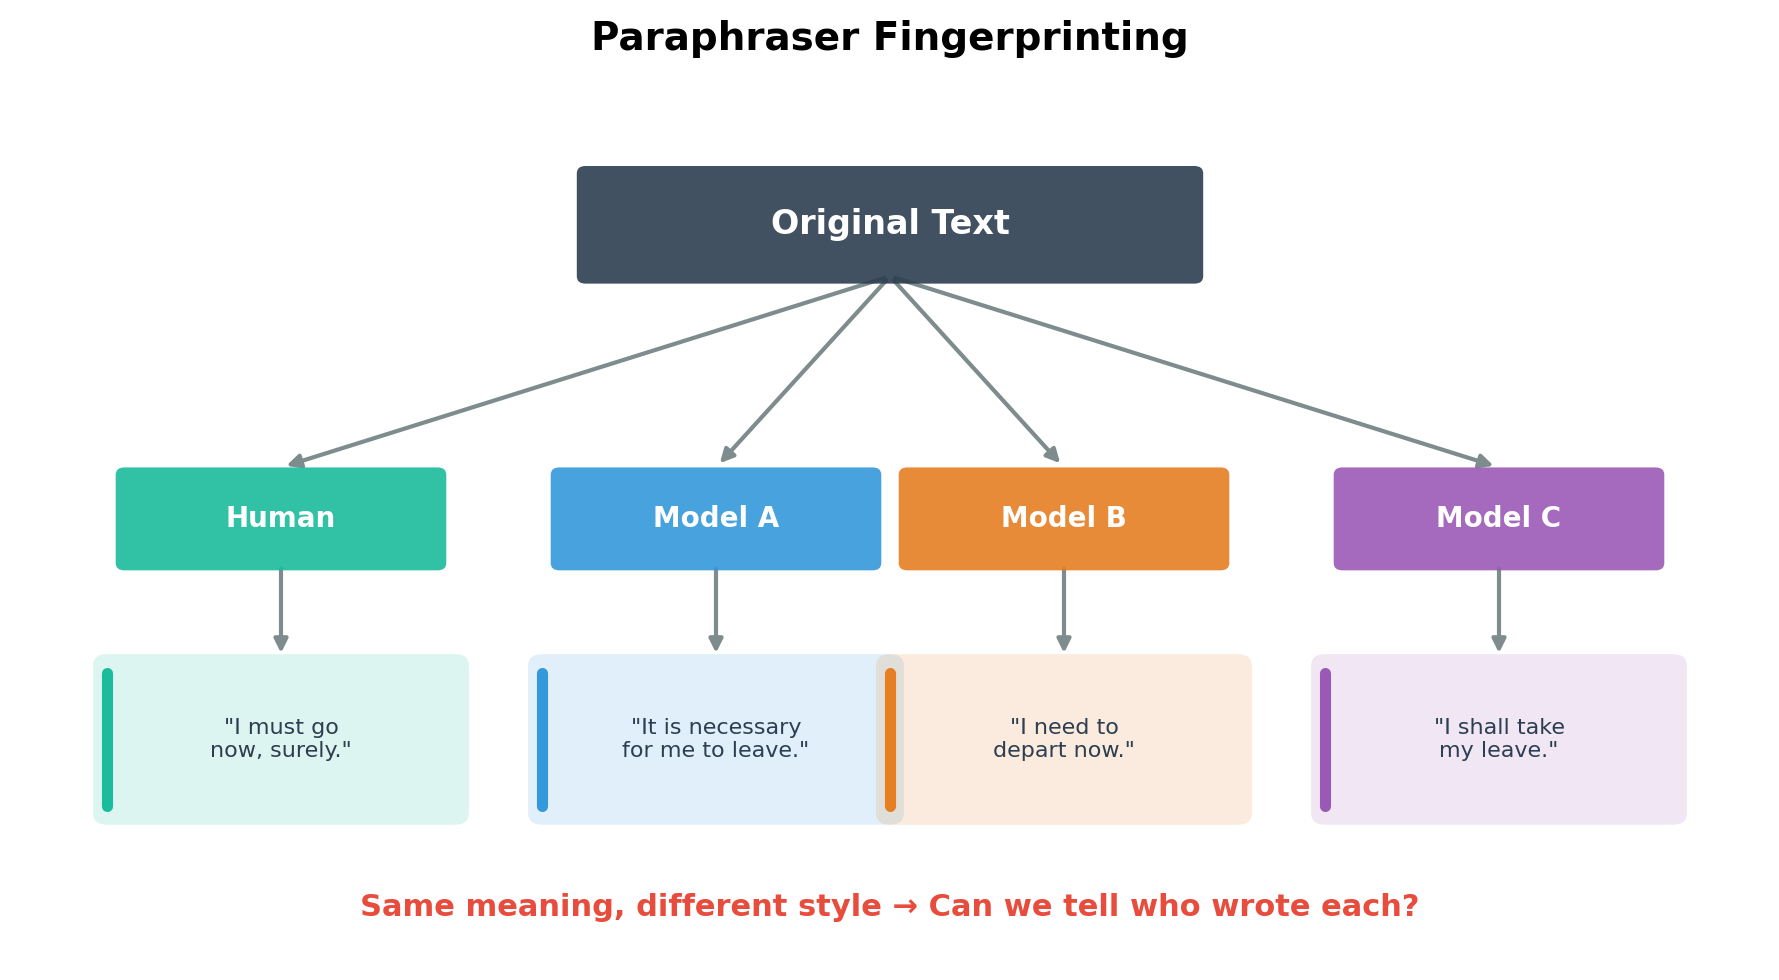
\includegraphics[width=0.82\linewidth]{figures/flow_motivation.png}
\end{center}
\vspace{-0.2cm}
\begin{itemize}
    \item Prior work: human vs.\ machine detection.
          \textbf{Our focus:} \emph{which} model wrote it?
    \item Applications: AI text detection, academic integrity, model provenance
\end{itemize}

\end{frame}

% ============================================================
\begin{frame}{Two Evaluation Paradigms}

\begin{columns}
\begin{column}{0.48\textwidth}
\textbf{Task 1: Duplicate Detection}
\begin{itemize}
    \item 4 paraphrasers, 1 source text
    \item One paraphraser writes \textbf{twice}
    \item 5 shuffled outputs
    \item Detective: ``Which 2 are from the same model?''
    \item Baseline: $\frac{1}{\binom{5}{2}} = 10\%$
\end{itemize}
\end{column}
\begin{column}{0.48\textwidth}
\textbf{Task 2: Pairwise Classification}
\begin{itemize}
    \item 4 paraphrasers, \textbf{2 source texts}
    \item Each model rewrites \textbf{both} texts
    \item 4+4 shuffled outputs
    \item Detective: ``Match pairs across groups''
    \item Baseline: $\frac{1}{4!} = 4.17\%$
\end{itemize}
\end{column}
\end{columns}

\end{frame}

% ============================================================
\begin{frame}{System Architecture --- Duplicate Detection}

\begin{center}
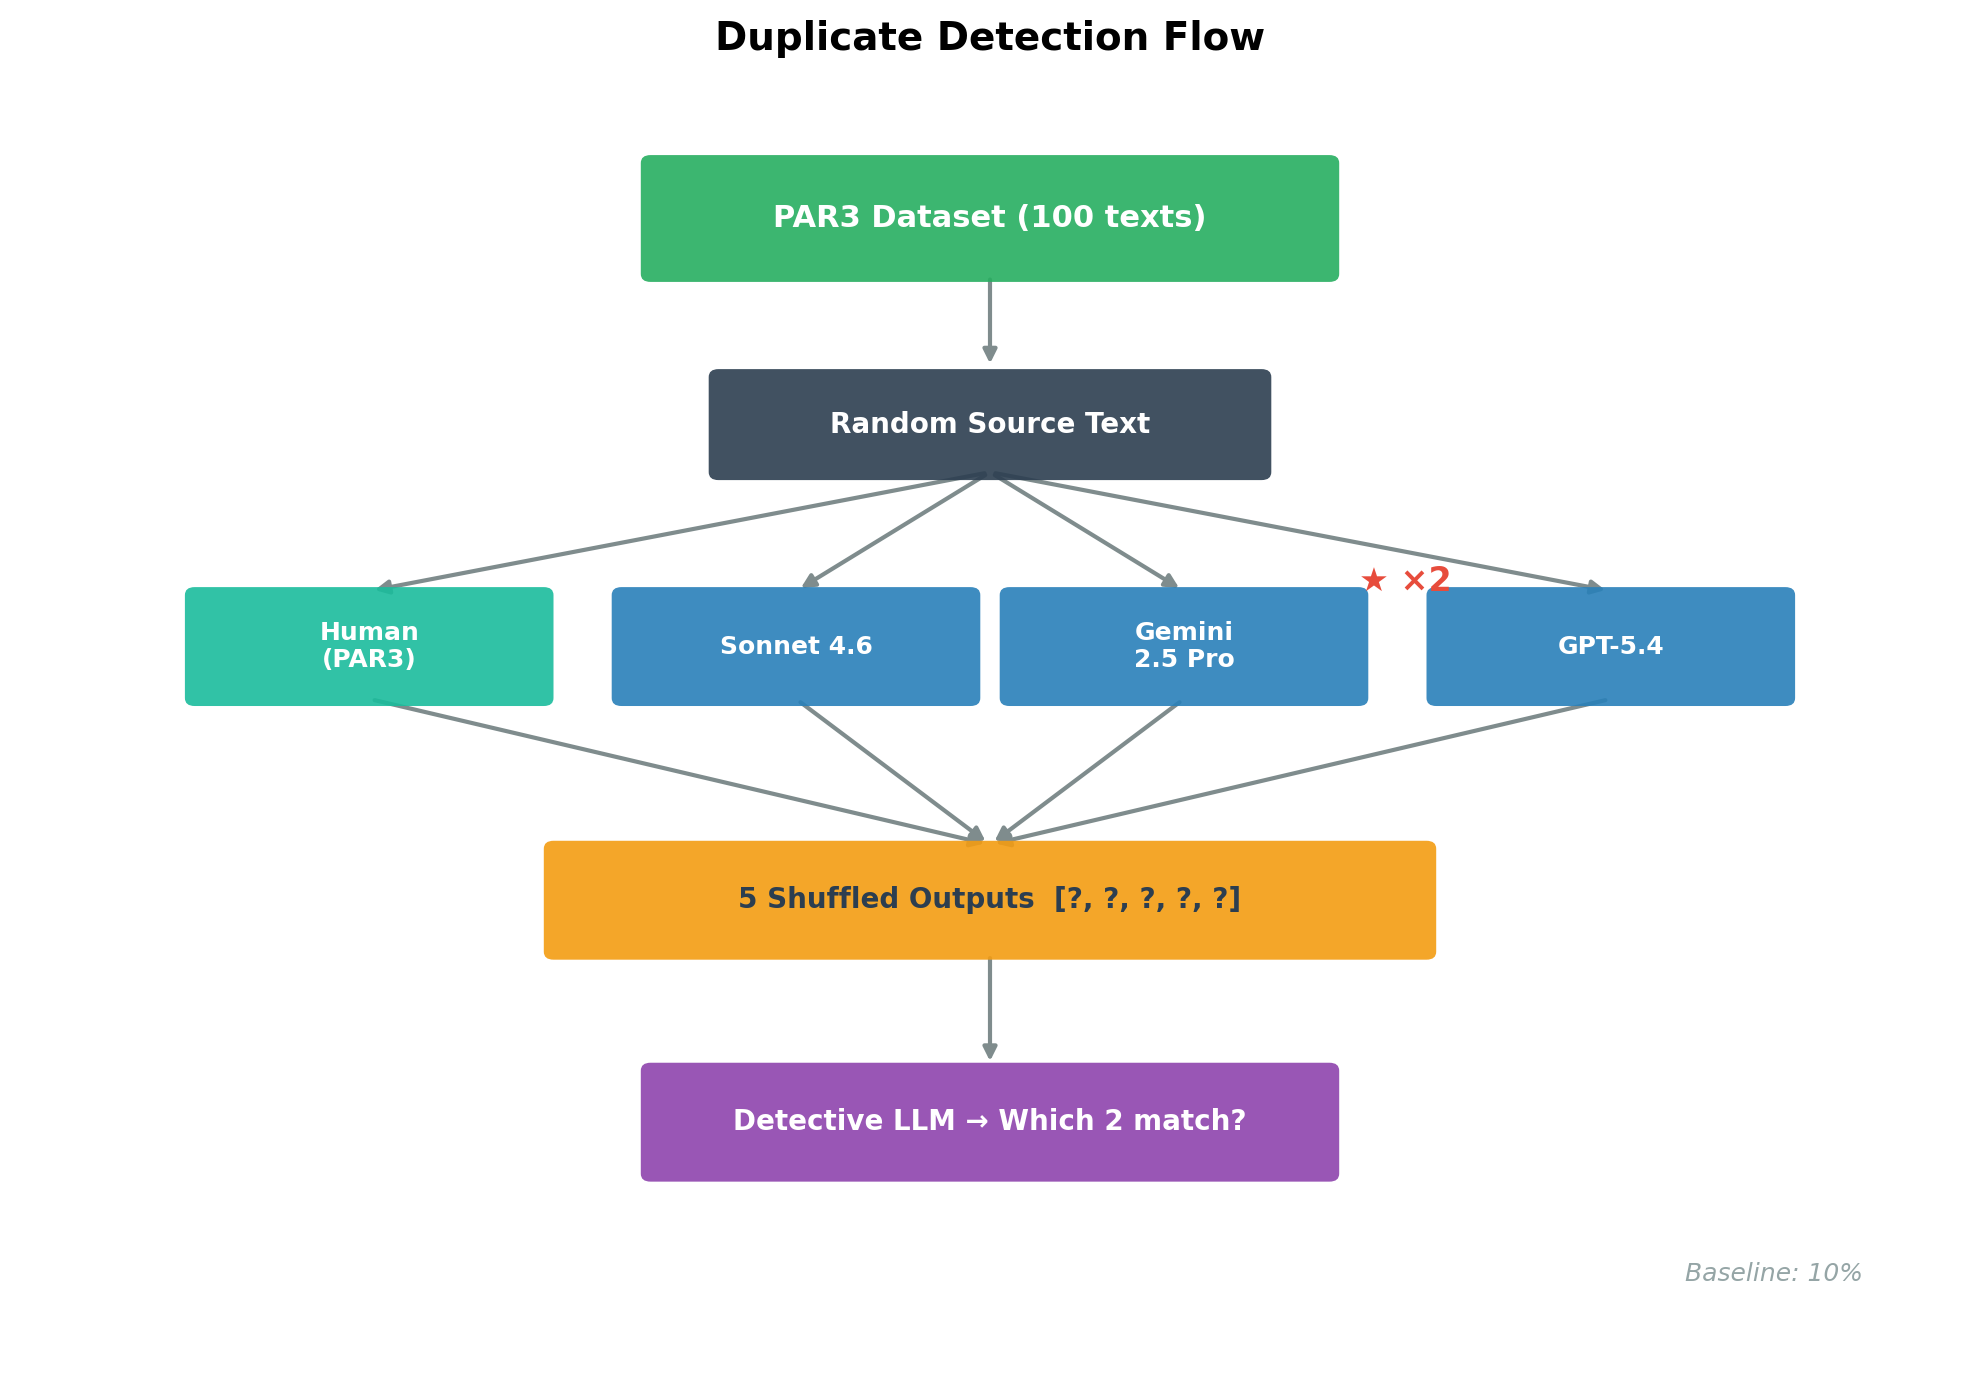
\includegraphics[width=0.85\linewidth]{figures/flow_duplicate.png}
\end{center}

\begin{itemize}
    \item Auditor randomly selects source text from PAR3 pool (100 texts)
    \item One paraphraser randomly chosen to produce 2 outputs
    \item Detective sees only current trial (no history)
\end{itemize}

\end{frame}

% ============================================================
\begin{frame}{System Architecture --- Pairwise Classification}

\begin{center}
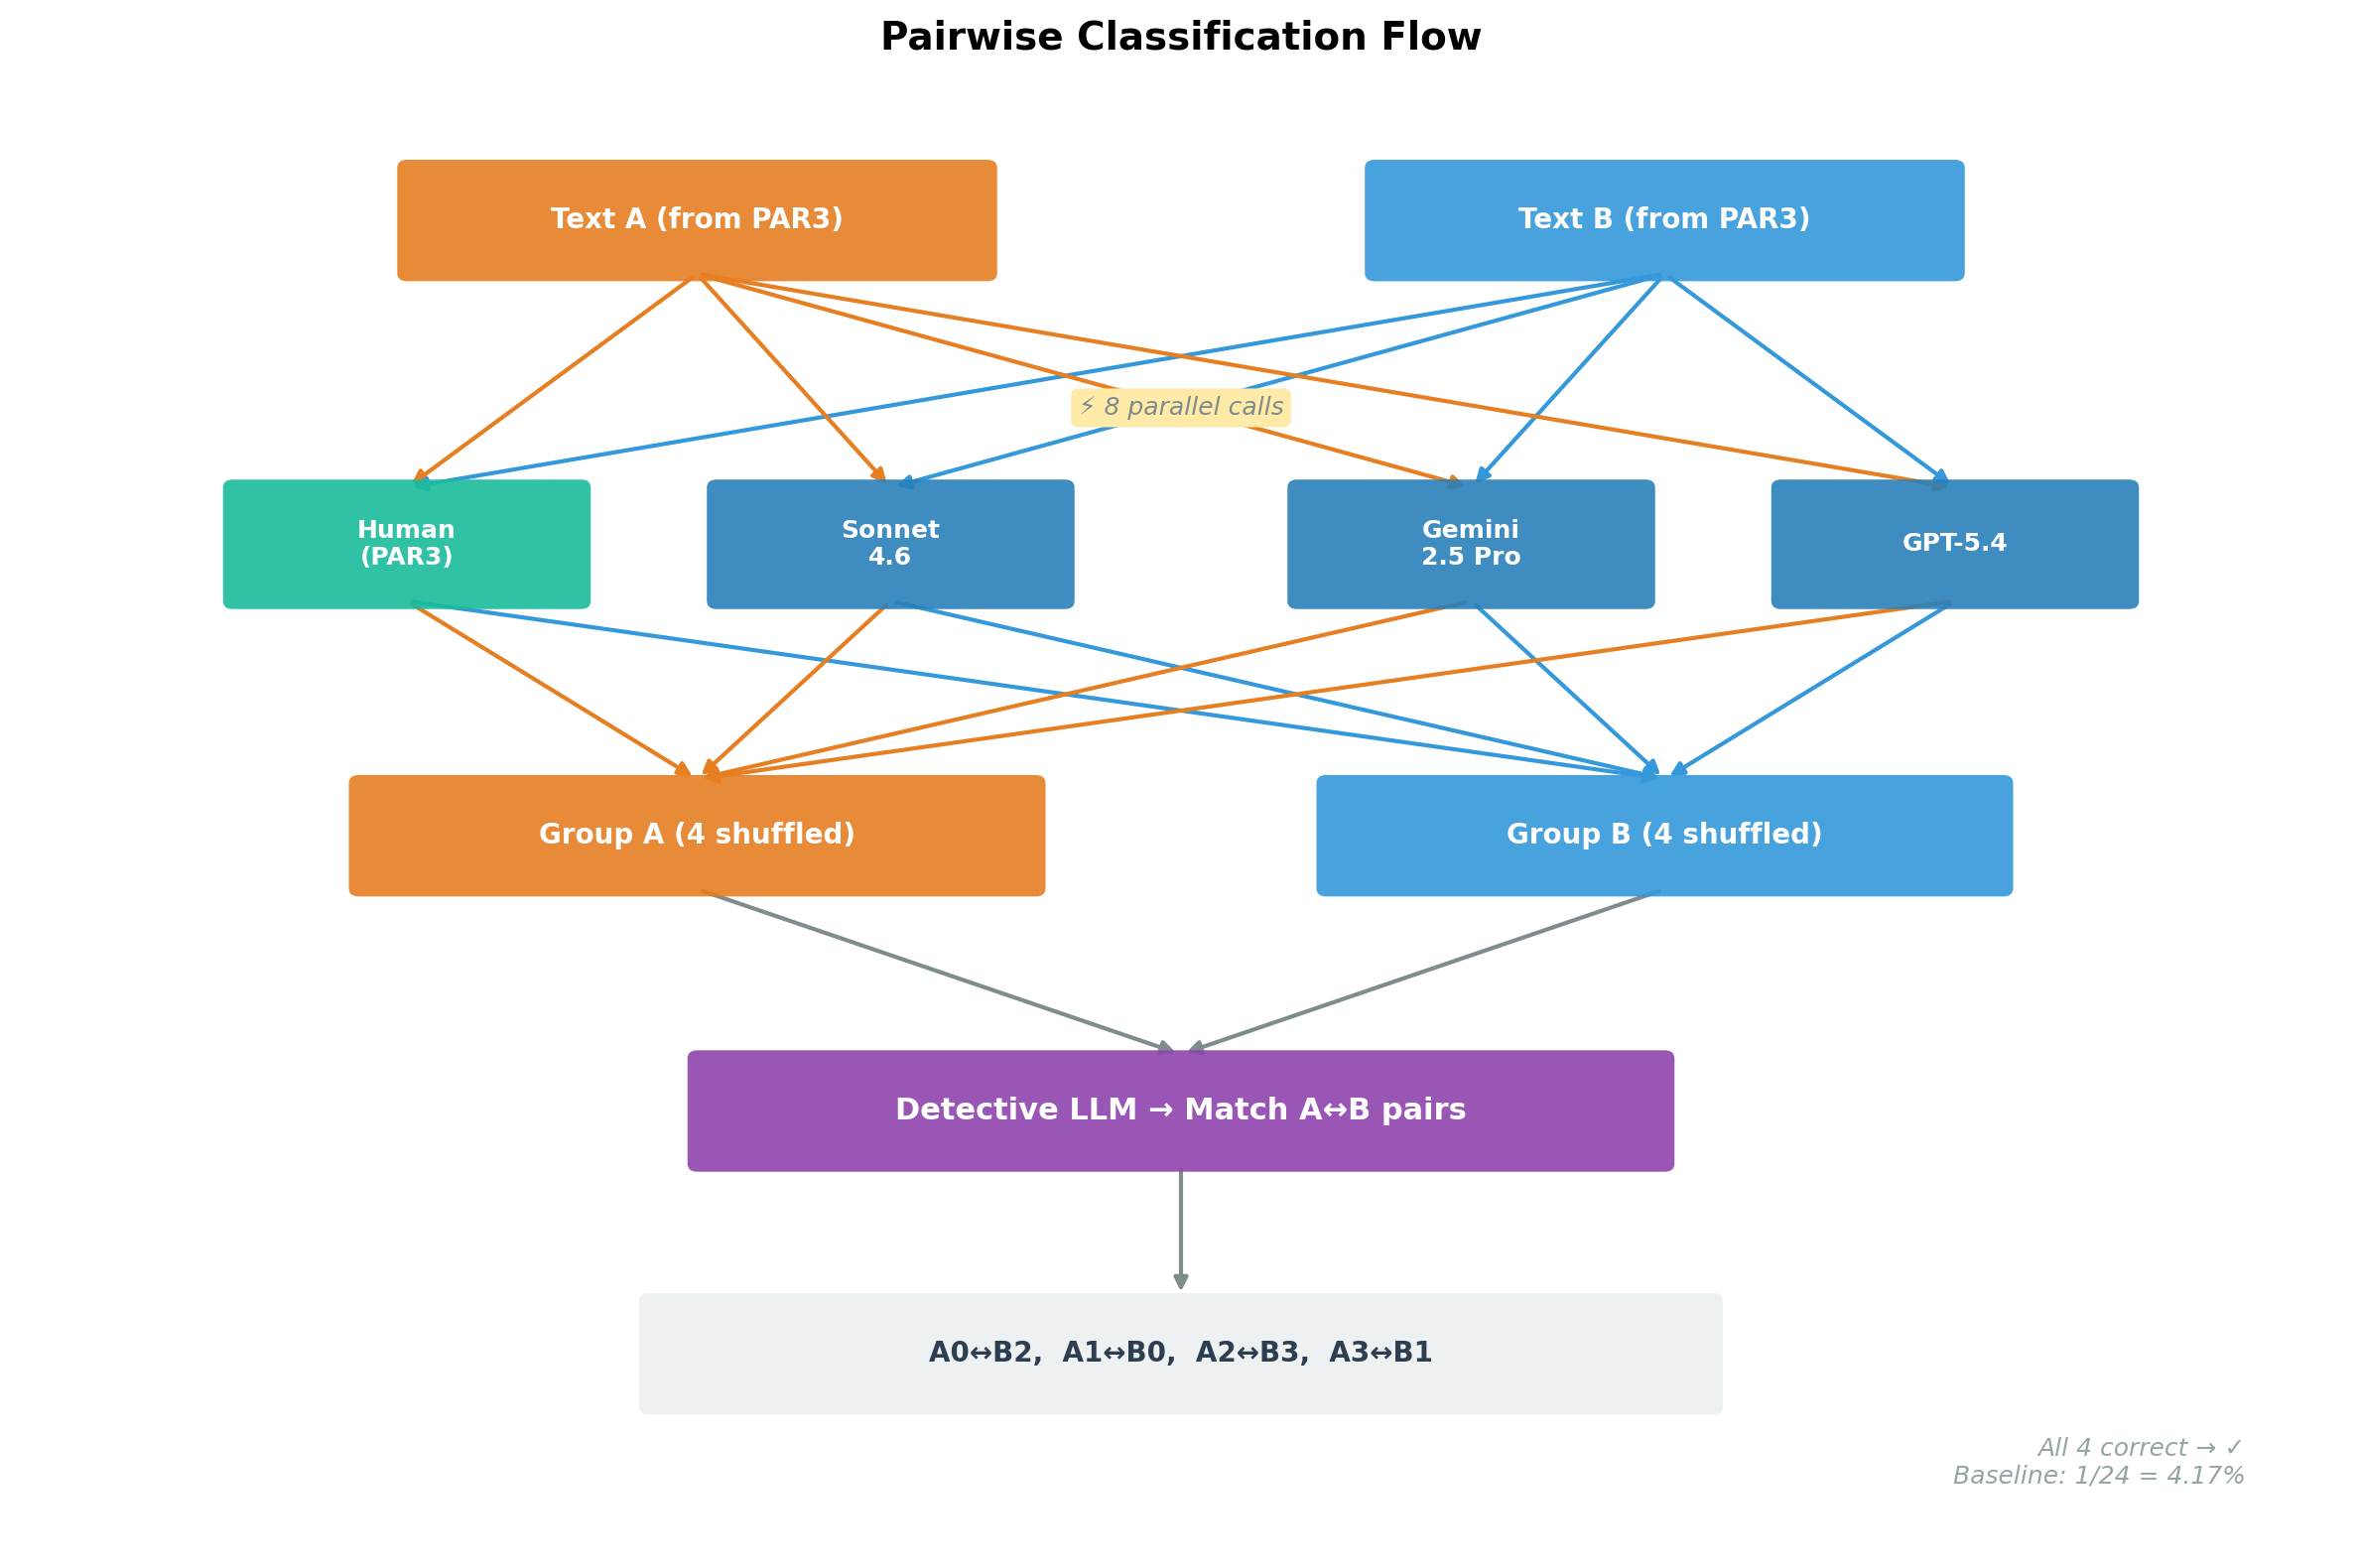
\includegraphics[width=0.85\linewidth]{figures/flow_classification.png}
\end{center}

\begin{itemize}
    \item Two texts drawn from PAR3; all 4 paraphrasers rewrite both
    \item 8 LLM calls parallelized (4 paraphrasers $\times$ 2 texts)
    \item Detective must produce a \textbf{complete permutation matching}
    \item Correct only if \textbf{all 4 matches} are right
\end{itemize}

\end{frame}

% ============================================================
\begin{frame}{Dataset: PAR3 Corpus}

\begin{center}
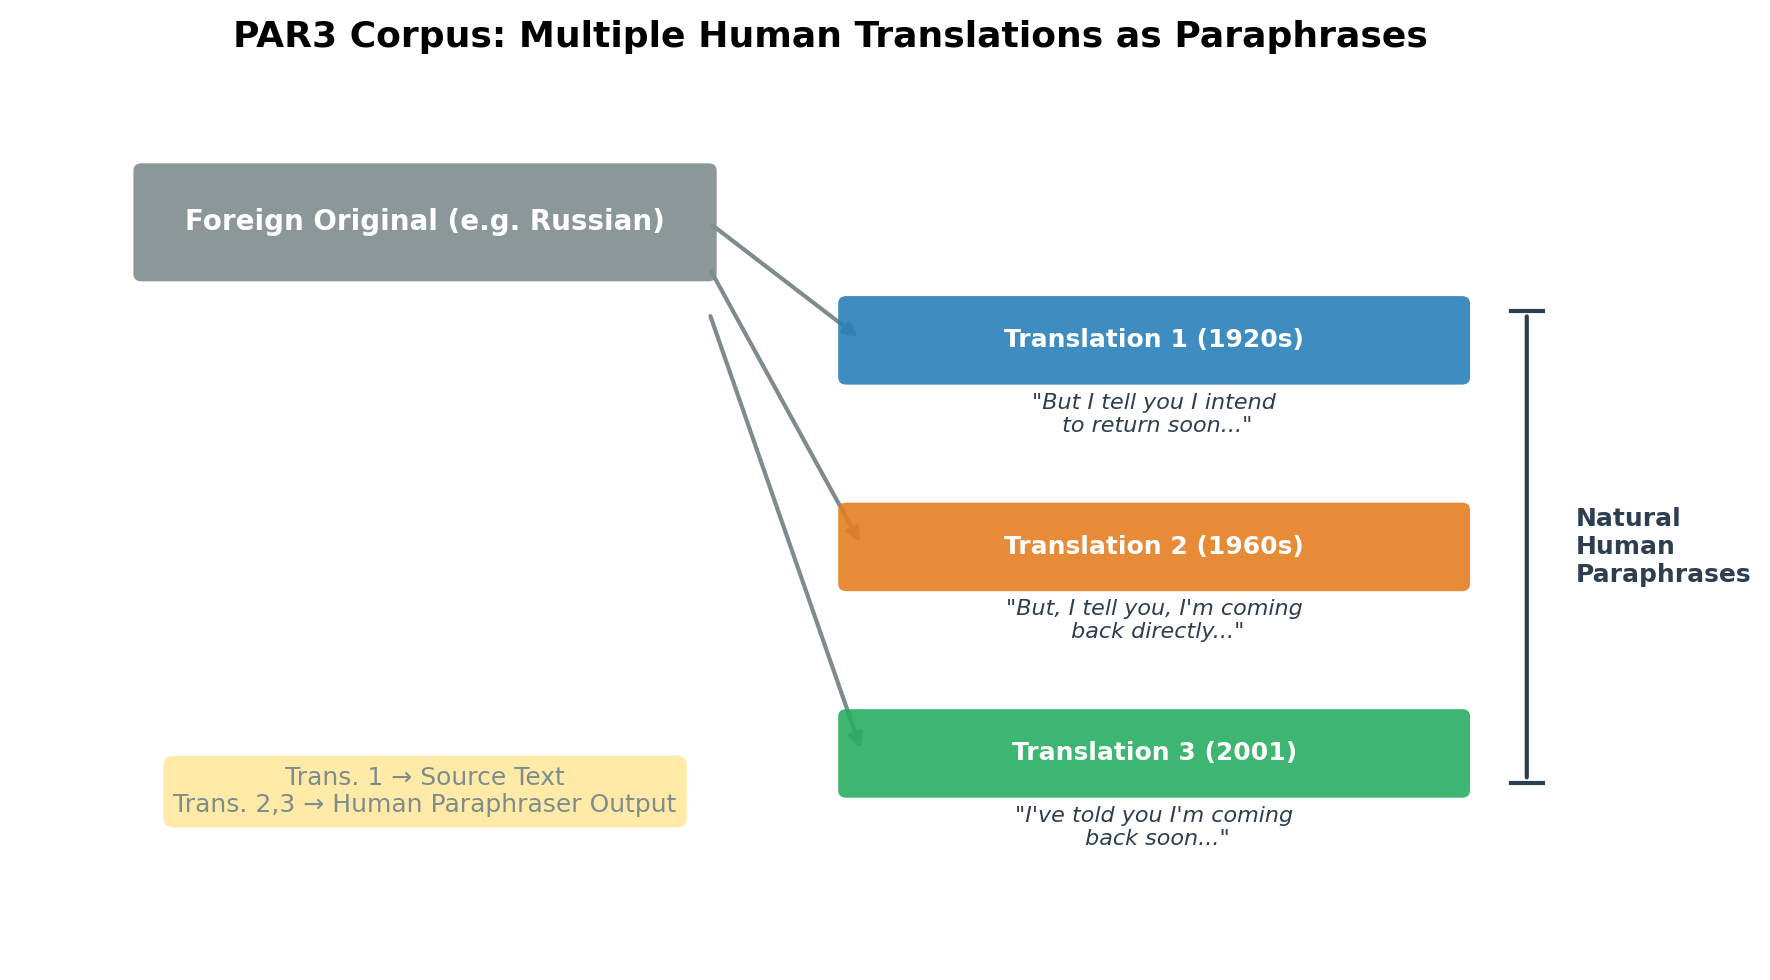
\includegraphics[width=0.78\linewidth]{figures/flow_par3.png}
\end{center}
\vspace{-0.2cm}
\begin{itemize}
    \item Multiple \textbf{human translations} of same paragraph $\Rightarrow$ natural paraphrases
    \item Sources: Dostoevsky, Voltaire, Verne, \ldots \quad Filter: $\geq 3$ translations, $\geq 100$ chars
\end{itemize}

\end{frame}

% ============================================================
\begin{frame}{Paraphraser Configurations}

\begin{columns}
\begin{column}{0.48\textwidth}
\textbf{``Weak'' Set}
\begin{itemize}
    \item Human (PAR3 translations)
    \item Llama-3.1-8B
    \item Gemini-2.5-Flash
    \item DIPPER (T5-based)
\end{itemize}
\vspace{0.3cm}
{\small Small/specialized models + human}
\end{column}
\begin{column}{0.48\textwidth}
\textbf{``Strong'' Set}
\begin{itemize}
    \item Human (PAR3 translations)
    \item Claude Sonnet 4.6
    \item Gemini 2.5 Pro
    \item GPT-5.4
\end{itemize}
\vspace{0.3cm}
{\small Frontier models + human}
\end{column}
\end{columns}

\vspace{0.5cm}
\begin{center}
\textbf{Detective models tested:} Sonnet 4.6, GPT-4.1, Gemini 2.5 Pro
\end{center}

\end{frame}

% ============================================================
\begin{frame}{Result 1: Duplicate Detection --- Detective Comparison}

\begin{columns}
\begin{column}{0.55\textwidth}
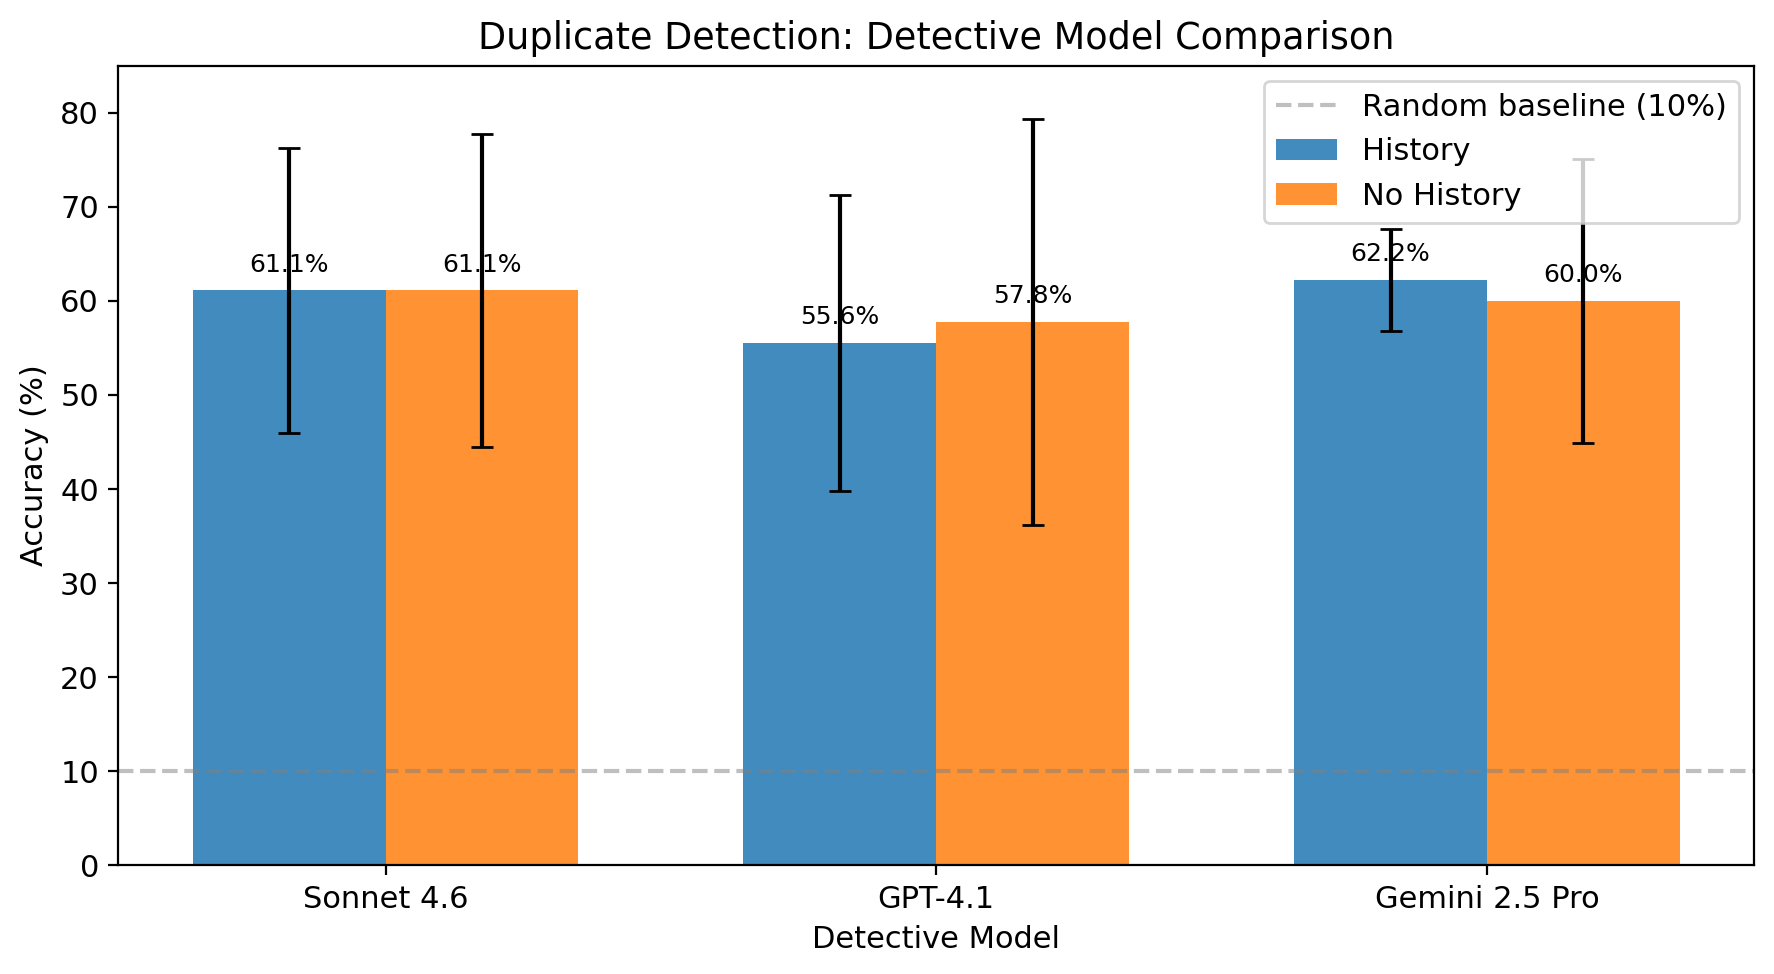
\includegraphics[width=\linewidth]{figures/fig3_detective_comparison.png}
\end{column}
\begin{column}{0.42\textwidth}
\begin{itemize}
    \item All detectives: \textbf{55--62\%} \\(baseline 10\%)
    \item \textbf{History does not help}\\Sonnet: 61.1\% $\leftrightarrow$ 61.1\%
    \item Gemini 2.5 Pro most consistent\\(SD = 5.4\%)
    \item 40+ runs, 400+ scored trials
\end{itemize}
\end{column}
\end{columns}

\end{frame}

% ============================================================
\begin{frame}{Result 2: Weak vs.\ Strong Paraphrasers}

\begin{columns}
\begin{column}{0.5\textwidth}
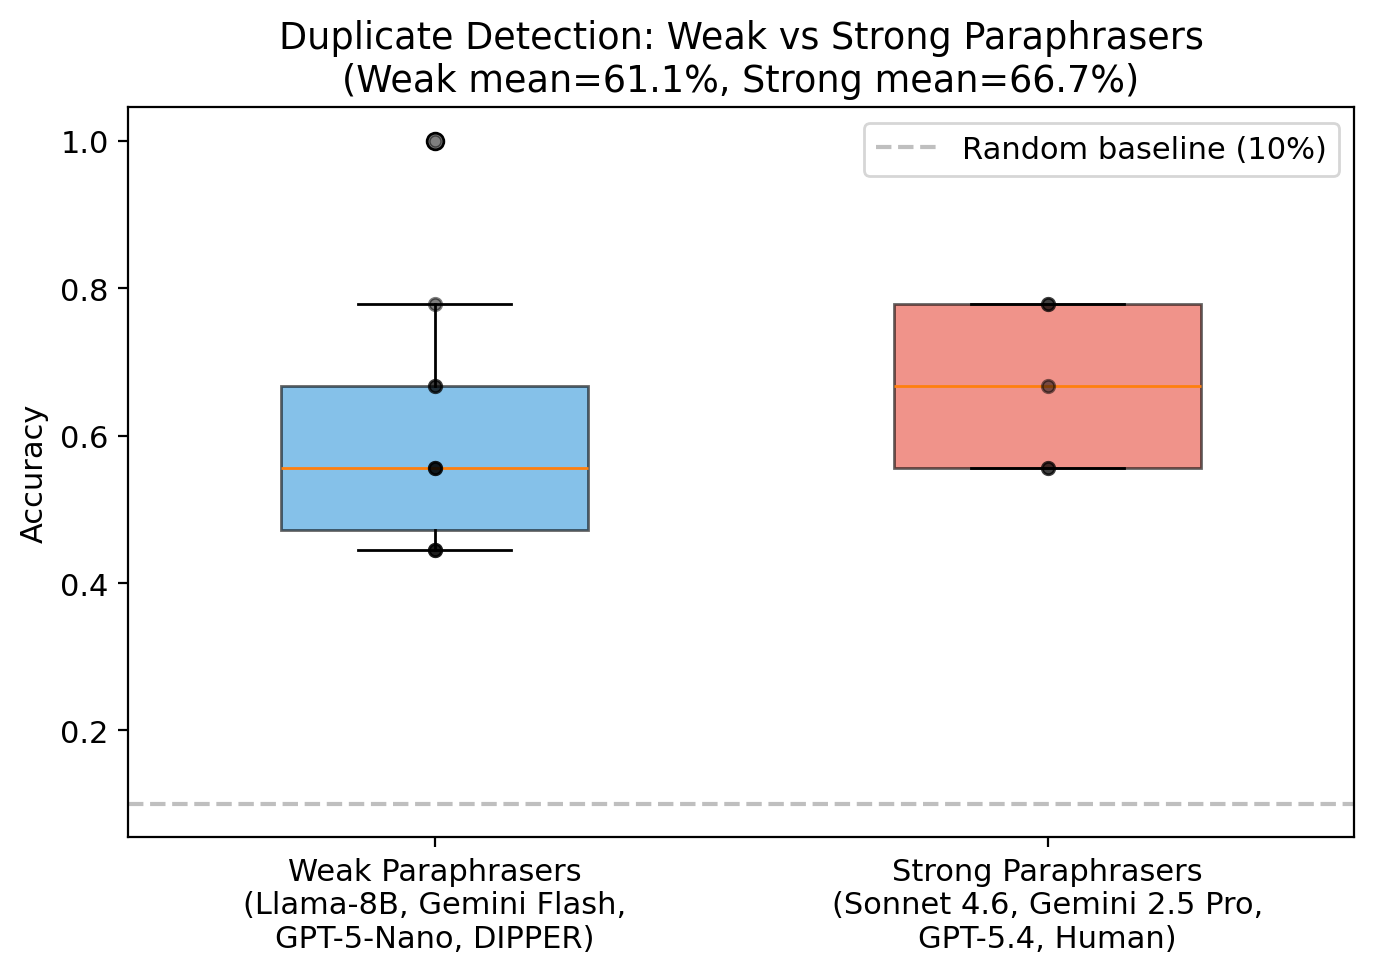
\includegraphics[width=\linewidth]{figures/fig4_weak_vs_strong.png}
\end{column}
\begin{column}{0.47\textwidth}
\textbf{Surprise:} Stronger models are \emph{easier} to detect!

\vspace{0.3cm}
\begin{tabular}{lc}
\toprule
\textbf{Set} & \textbf{Mean Acc.} \\
\midrule
Weak  & 61.1\% \\
Strong & \textbf{66.7\%} \\
\bottomrule
\end{tabular}

\vspace{0.3cm}
\textbf{Why?} Capable models develop more consistent ``voices'' --- stronger fingerprints
\end{column}
\end{columns}

\end{frame}

% ============================================================
\begin{frame}{Result 3: Pairwise Classification --- Main Result}

\begin{center}
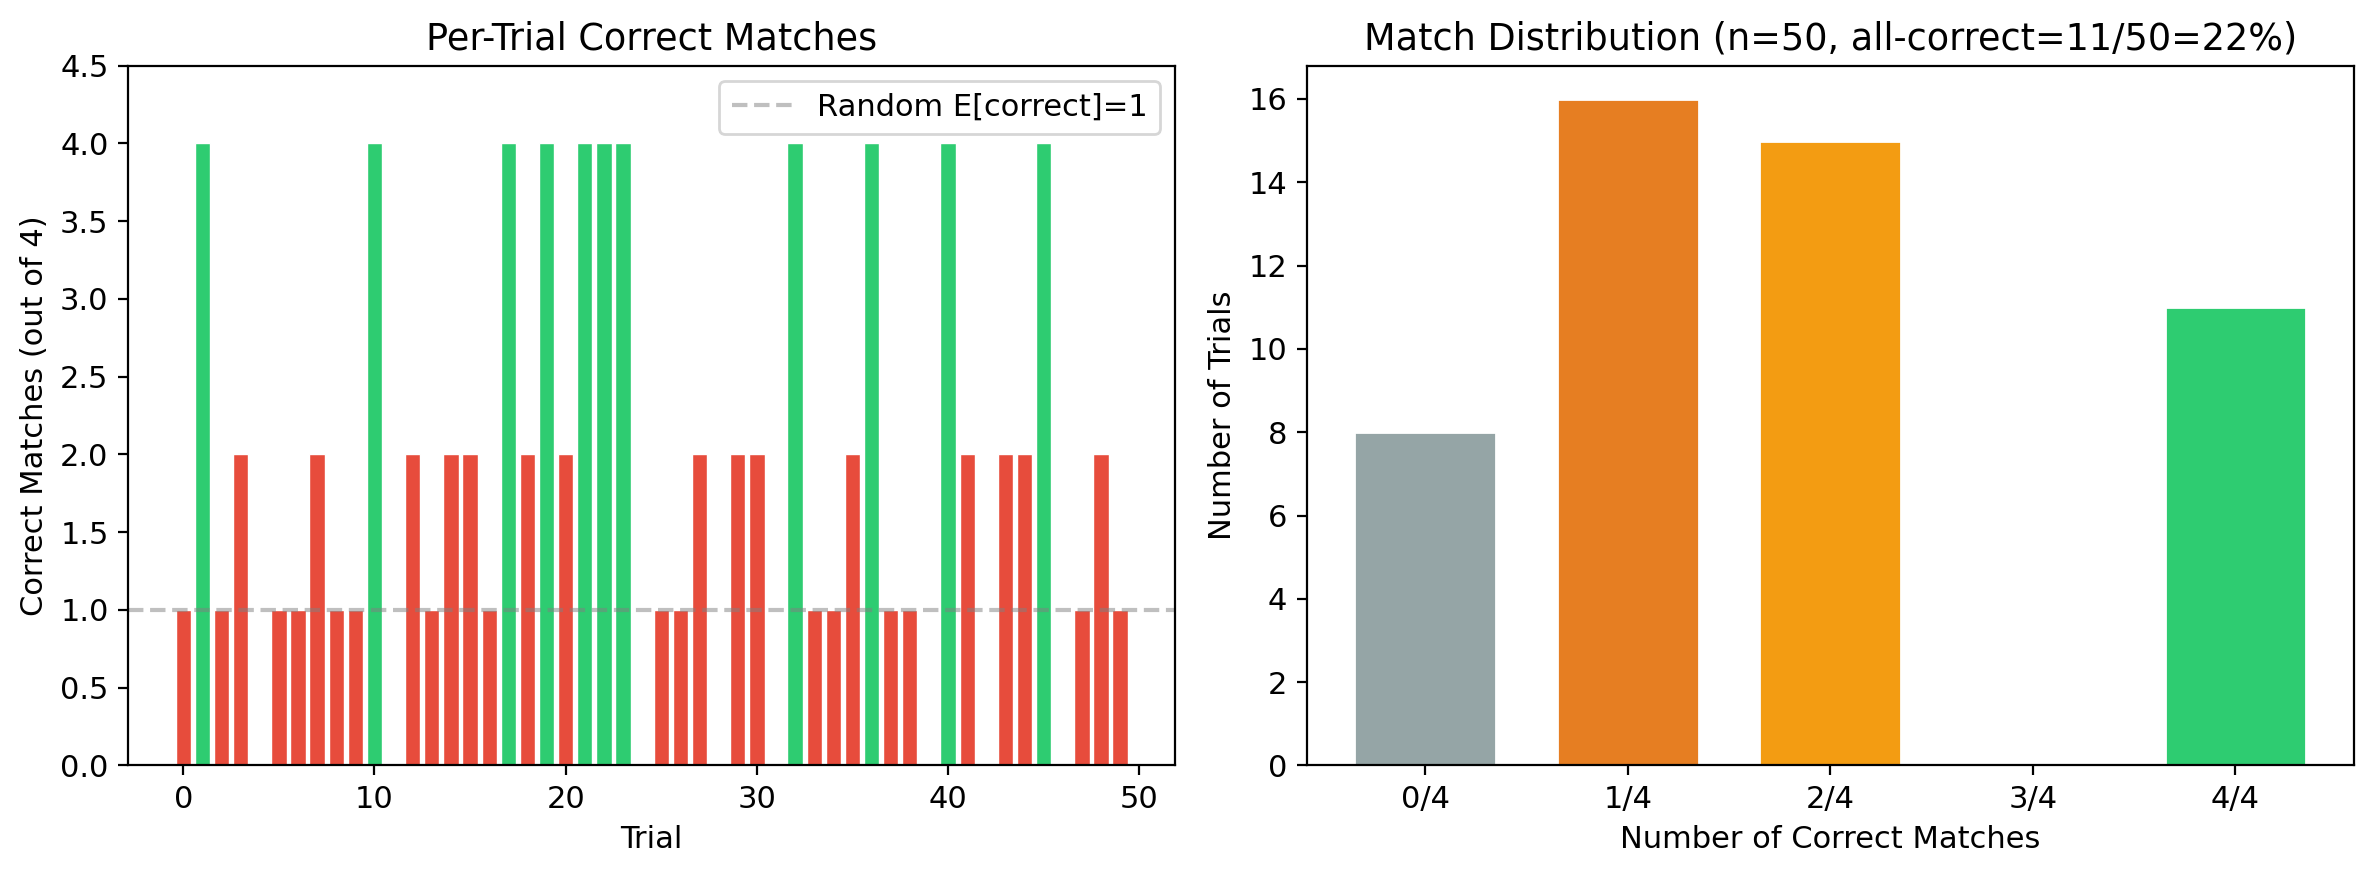
\includegraphics[width=0.95\linewidth]{figures/fig1_classification_main.png}
\end{center}

\begin{columns}
\begin{column}{0.5\textwidth}
\begin{itemize}
    \item \textbf{22\%} perfect match (11/50)
    \item Baseline: 4.17\% $\Rightarrow$ \textbf{5.3$\times$}
\end{itemize}
\end{column}
\begin{column}{0.5\textwidth}
\begin{itemize}
    \item \textbf{Bimodal:} 0 trials with 3/4
    \item Either all-correct or multiple errors
\end{itemize}
\end{column}
\end{columns}

\end{frame}

% ============================================================
\begin{frame}{Result 4: Who Is Most Identifiable?}

\begin{columns}
\begin{column}{0.5\textwidth}
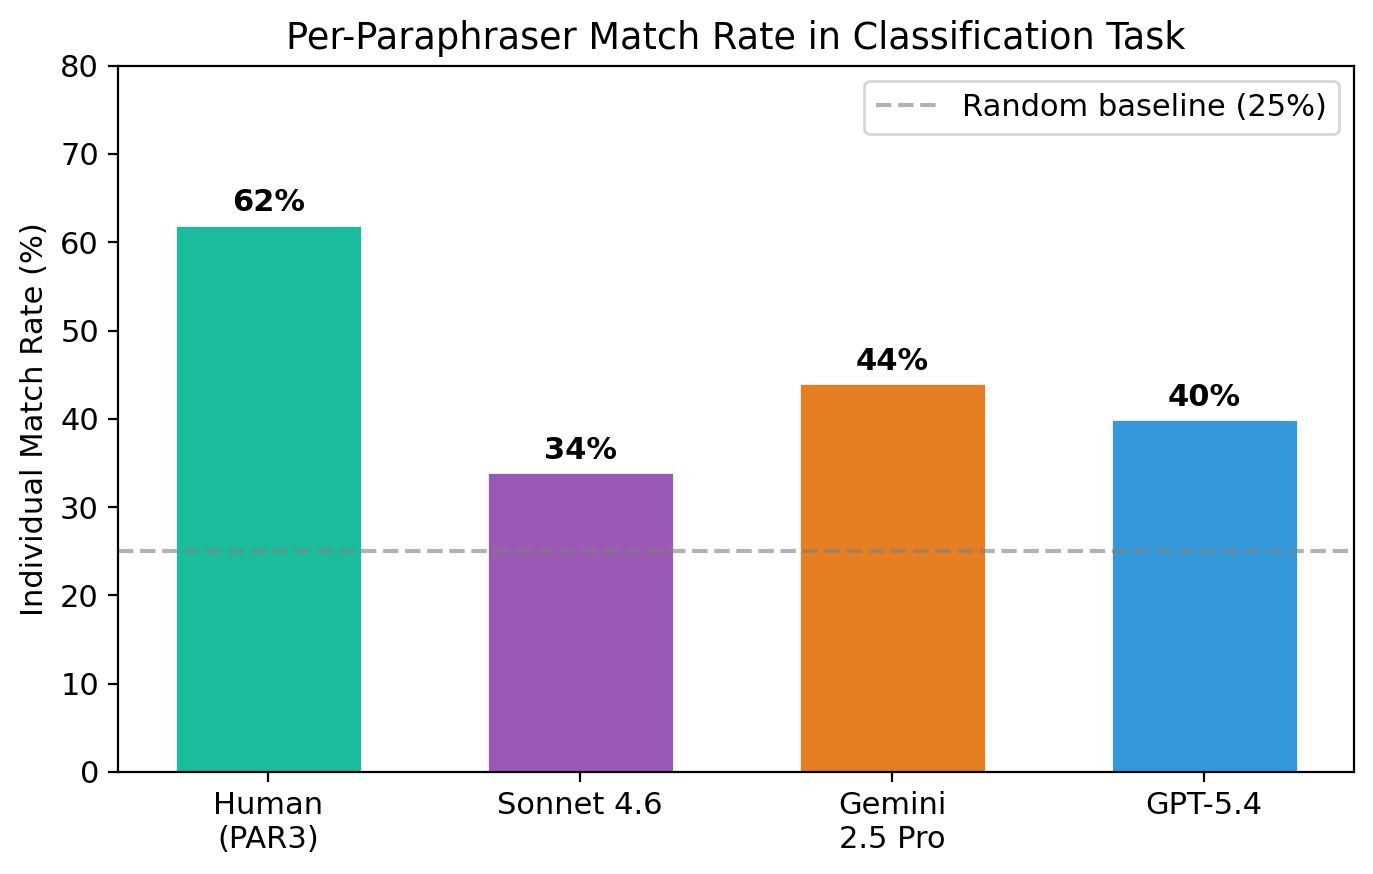
\includegraphics[width=\linewidth]{figures/fig2_paraphraser_matchrate.png}
\end{column}
\begin{column}{0.47\textwidth}
\begin{tabular}{lc}
\toprule
\textbf{Paraphraser} & \textbf{Match Rate} \\
\midrule
\textcolor{success}{Human (PAR3)} & \textbf{62\%} \\
Gemini 2.5 Pro & 44\% \\
GPT-5.4 & 40\% \\
\textcolor{highlight}{Sonnet 4.6} & 34\% \\
\midrule
Random & 25\% \\
\bottomrule
\end{tabular}

\vspace{0.3cm}
\textbf{Key finding:}\\
Humans are the \emph{most} identifiable!\\
Sonnet 4.6 is the best ``disguiser''
\end{column}
\end{columns}

\end{frame}

% ============================================================
\begin{frame}{Result 5: Confusion Matrix}

\begin{columns}
\begin{column}{0.52\textwidth}
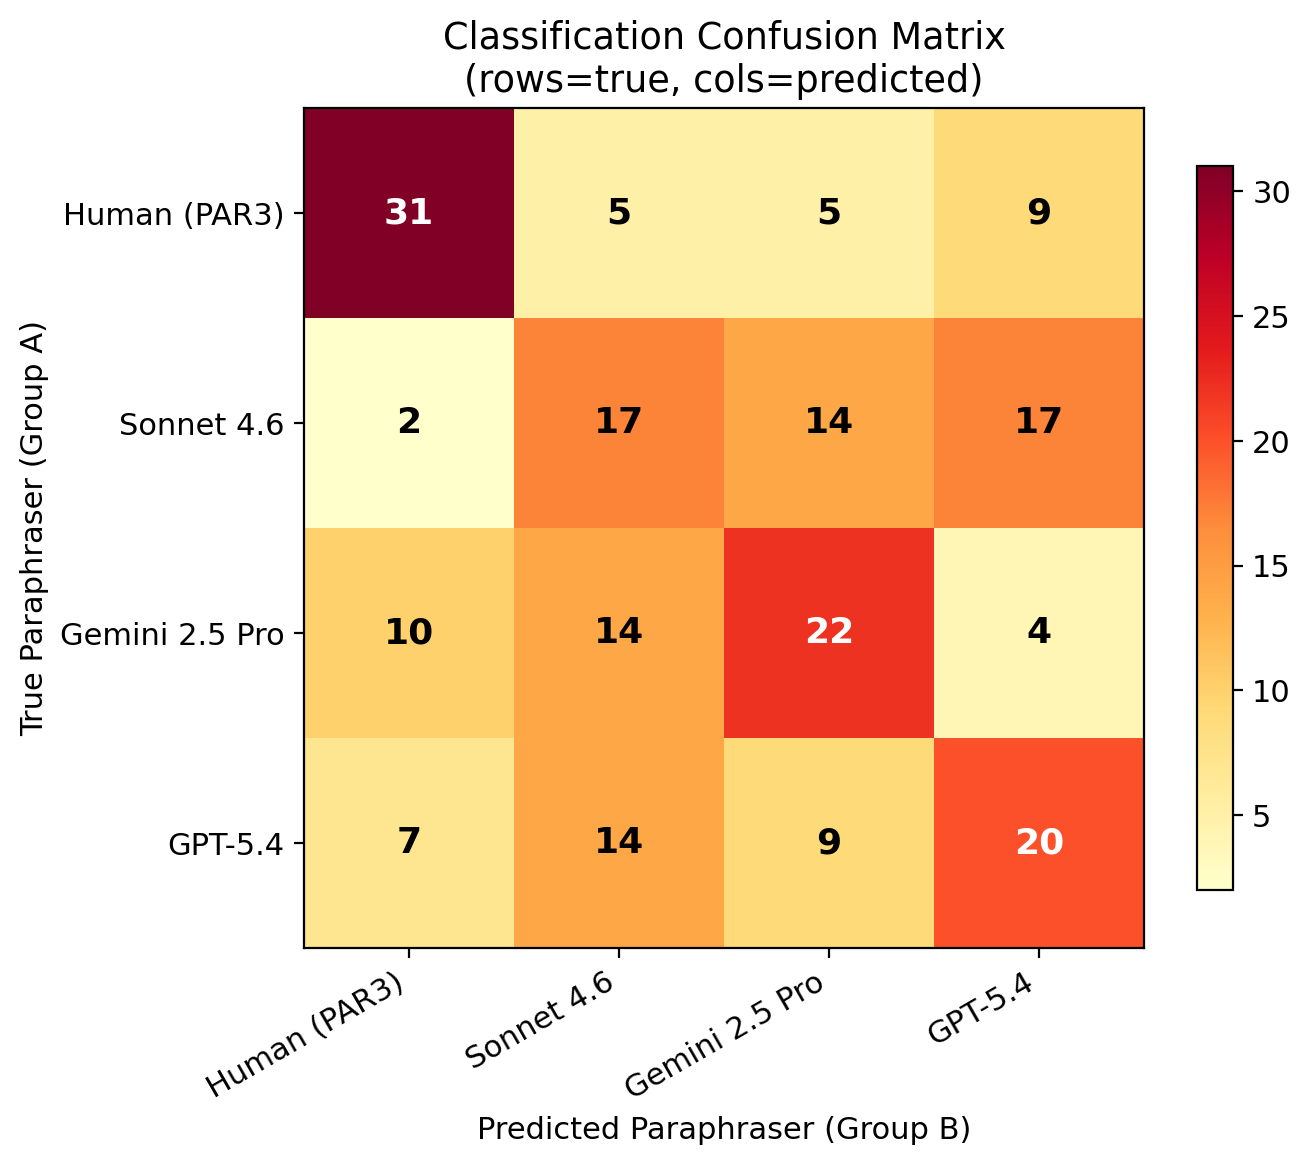
\includegraphics[width=\linewidth]{figures/fig6_classification_confusion.png}
\end{column}
\begin{column}{0.45\textwidth}
\begin{itemize}
    \item Human rarely confused with LLMs
    \item LLMs frequently confused with each other
    \item Human fingerprint occupies a \textbf{distinct region} of style space
    \item Sonnet 4.6 most ``generic'' --- hardest to pin down
\end{itemize}
\end{column}
\end{columns}

\end{frame}

% ============================================================
\begin{frame}{Experimental Summary}

\begin{center}
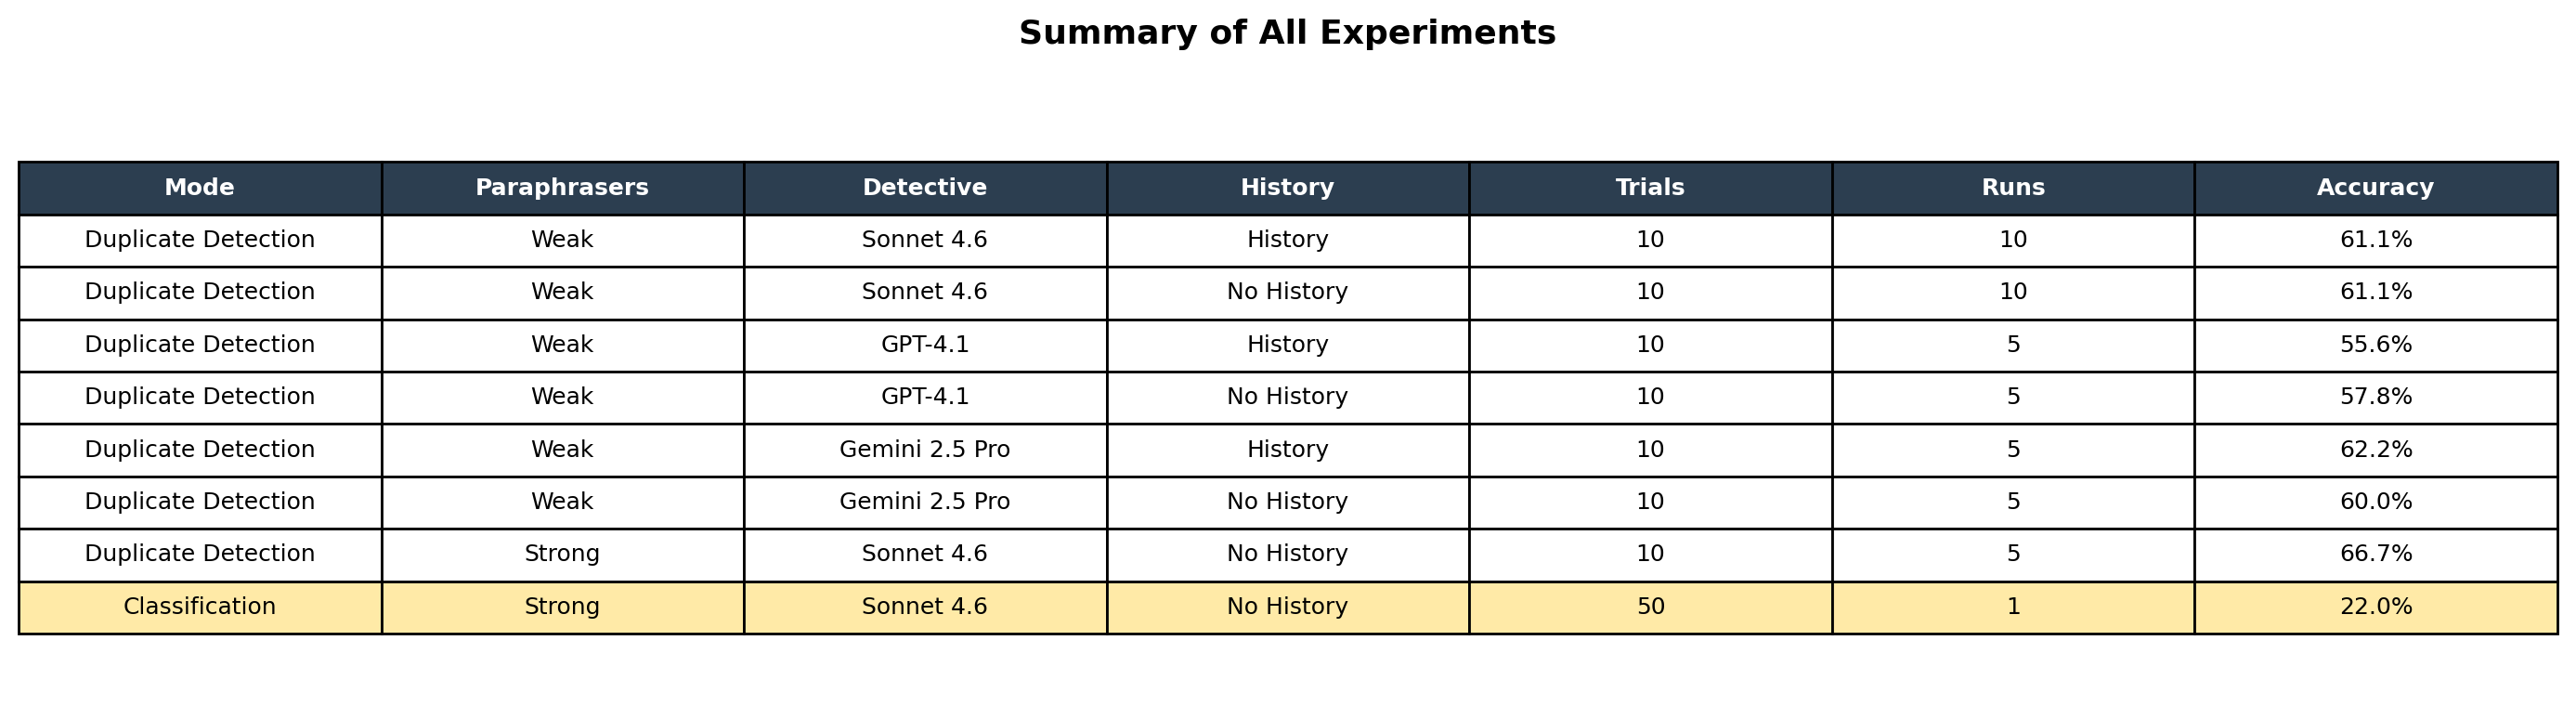
\includegraphics[width=0.92\linewidth]{figures/fig5_summary_table.png}
\end{center}

\vspace{0.2cm}
{\small 8 configurations $\cdot$ 50+ runs $\cdot$ 500+ scored trials}

\end{frame}

% ============================================================
\begin{frame}{Key Takeaways}

\begin{enumerate}
    \item \textbf{Fingerprints are real.}\\
    All conditions far exceed random baselines (6$\times$ for duplicate, 5.3$\times$ for classification)

    \vspace{0.2cm}
    \item \textbf{Humans are most identifiable.}\\
    PAR3 human translations: 62\% match rate vs.\ 34--44\% for LLMs

    \vspace{0.2cm}
    \item \textbf{Stronger models $=$ stronger fingerprints.}\\
    Frontier LLMs develop more distinctive ``voices'' (66.7\% vs.\ 61.1\%)

    \vspace{0.2cm}
    \item \textbf{History doesn't help.}\\
    Within-trial stylistic comparison matters more than cross-trial memory

    \vspace{0.2cm}
    \item \textbf{Pairwise classification is hard but feasible.}\\
    22\% perfect match with bimodal success pattern
\end{enumerate}

\end{frame}

% ============================================================
\begin{frame}{Future Work}

\begin{itemize}
    \item \textbf{Scale paraphraser pool:} 8+ models, same-family comparison (e.g., Llama-8B vs.\ Llama-70B)
    \item \textbf{Feature-based classifier:} Complement LLM detective with traditional NLP features (n-grams, syntax)
    \item \textbf{Robustness:} Do fingerprints survive post-processing (grammar correction, back-translation)?
    \item \textbf{Cross-domain:} Test across scientific, literary, conversational text
    \item \textbf{Embedding analysis:} Use embedding similarity as a quantitative fingerprint metric
\end{itemize}

\end{frame}

% ============================================================
\begin{frame}{}
\begin{center}
{\Huge Thank You}

\vspace{1cm}
{\large Questions?}

\vspace{1cm}
{\small Code: \url{https://github.com/zboyr/HideNSeek}}
\end{center}
\end{frame}

\end{document}
